\section{\label{III-A-2}Les solutions techniques existantes : entre standardisation et adaptation locale}


La maîtrise de la prolifération documentaire ne saurait être réduite à une question de modélisation conceptuelle : elle implique le choix raisonné d’outils susceptibles d’articuler la complexité du réel, tout en répondant à des contraintes de gouvernance, d’interopérabilité et de pérennité. Nous nous sommes attachés dans ce mémoire à l'analyse de deux grandes catégories de l'information qui se retrouve dans un musée : celle qui est utilisée pour décrire ses collections, en la matière des thésaurus et vocabulaires contrôlés aujourd'hui présents au musée, et celle qu'il produit quotidiennement dans le cadre de on activité en tant qu'institution publique avec ses archives numériques. Des outils, techniques comme conceptuels, existent pour aider à la structuration et à la diffusion de cette information : nous avons évoqué, pour les archives numérique, l'utilité du respect de normes nationales et d'outils numériques comme une \gls{ged} ou un \ac{sae}. Pour la gestion des vocabulaires contrôlés, c'est un autre outil de modélisation de la connaissance qui s'est imposé : le thésaurus documentaire.



\subsection{\label{III-A-2.1}Qu’est-ce qu’un thésaurus documentaire ?}

On ne peut réduire le thésaurus documentaire à une simple liste de mots ou à un instrument technique. La norme ISO 25964, qui fait aujourd’hui autorité, le définit comme un \enquote{vocabulaire contrôlé et structuré dans lequel les concepts sont représentés par des termes, organisés de façon à ce que des relations entre les concepts soient explicitées, et dont les termes préférentiels sont accompagnés par des entrées vers leurs synonymes ou quasi-synonymes}\footcite{ISO25964120112011,maroyeISO25964Distinction2015}. Celui-ci ne se contente donc pas d’indexer, il articule une vision du monde, une manière de penser le réel à travers le langage documentaire. Il impose donc notamment :
\begin{itemize}
	\item de distinguer le concept (une idée), du terme (le mot choisi pour l'exprimer),
	\item de choisir un terme préféré qui servira à décrire le concept,
	\item de mettre les autres termes en synonymes (\textbf{relations d'équivalence})
	\item des \textbf{relations hiérarchiques} avec :
		\subitem des termes génériques,
		\subitem des termes spécifiques ;
	\item des \textbf{relations d'association} entre les termes,
	\item des définitions, notes et alignements externes associés aux termes.
\end{itemize}

Comme montré dans l'image suivante, la structuration d’un thésaurus suppose ainsi une modélisation précise : chaque concept est relié à des termes, chaque terme préféré est accompagné de notes explicatives, chaque branche de la hiérarchie répond à des logiques de genre à espèce, de tout à partie ou  d'instance à classification\footnote{Pour plus de précisions, consulter l'article suivant \cite{perrinBonnesPratiquesPour2020}}. Cette méthode permet notamment de multiplier les accès à l'information, et de faire entrer en adéquation le langage de l'utilisateur avec le langage de l'institution. 

\begin{figure}
	\centering
	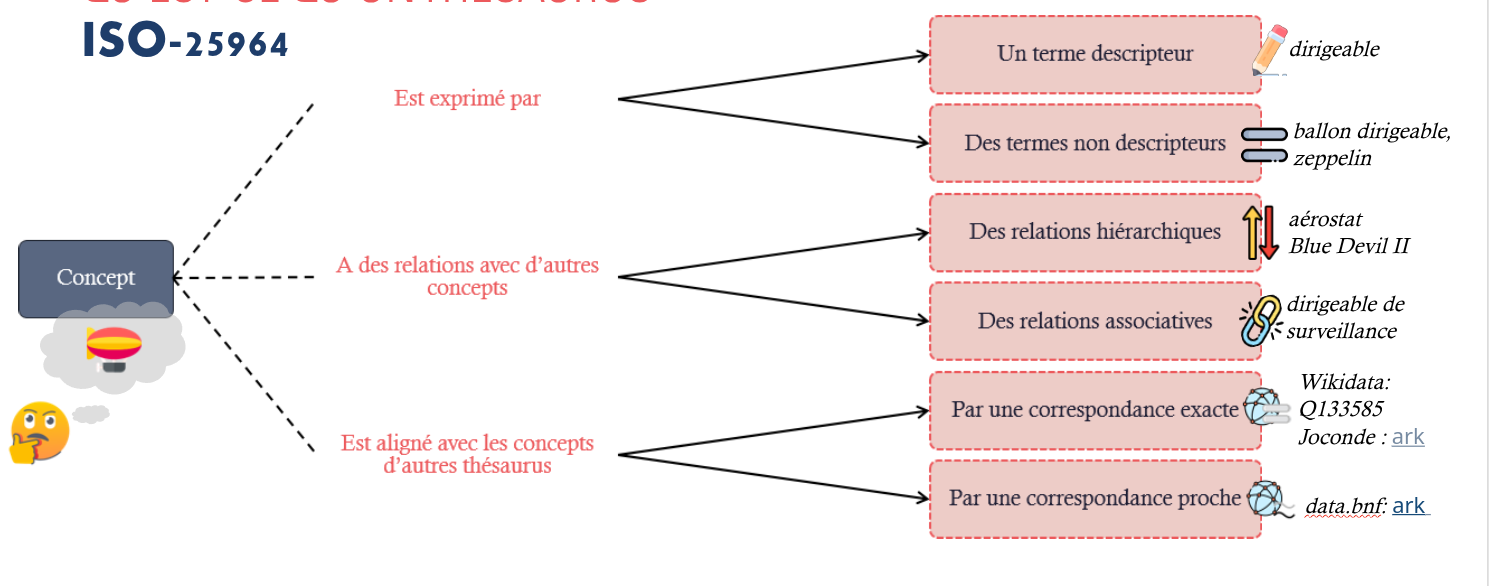
\includegraphics[width=0.9\linewidth]{img/SCHEM_thesaurus}
	\caption[Relations sémantiques exprimées par un thésaurus]{L'ensemble des relations sémantiques exprimées par un thésaurus. \textit{Schéma utilisé dans la formation du 4 juin 2025, inspiré de \protect\cite{perrinBonnesPratiquesPour2020}}.}
	\label{fig:schemthesaurus}
\end{figure}


\subsection{Diversité des outils de structuration de l’information}

Simple et efficace, le \gls{thesaurus} s'est imposé au \mae comme un outil compatible avec les logiciels métiers utilisés. Au fil des réflexions sur leur réorganisation, sont cependant apparues diverses difficultés : il est en effet apparu que le \gls{thesaurus} ne permettrait pas d'englober l'ensemble des connaissances requises au musée pour gérer ses collections. En effet, un thésaurus reste un outil lexical, qui permet de contrôler la description des objets : il ne permet pas, par exemple, de symboliser des liens de famille entre des personnes enregistrées comme terme ou d'expliciter les types de relations -- auteur, constructeur, utilisé dans... -- entre deux termes associés.
Il est apparu que pour arriver à cette granularité d'information, un autre outil devrait être adopté : l'ontologie documentaire. Pour citer Thomas Francart, expert dans les systèmes de gestion des connaissances et fondateur de la société SPARNA, \blockquote{l’ontologie cherche à décrire de façon formelle un domaine de connaissance, en identifiant les types d’objets de ce domaine, leurs propriétés et leurs relations\footcite{francartOntologieThesaurusTaxonomie2013}.}

Bien plus riche que le thésaurus, ce format pourrait répondre aux besoins diversifiés du \mae en lui permettant de couvrir davantage de connaissances, et de mieux adresser la diversité de ses utilisateurs avec un système plus modulables que le thésaurus : sa mise en place demanderait cependant un travail de restructuration, de recherche et de création de liens considérable.

C'est le choix qui a été fait par d'autres institutions devant répondre à des exigences similaires : pour ne pas citer le cas bien connu de la \ac{bnf}, citons par exemple celui de la fondation SAPA -- Archives suisses des arts de la scène qui a migré en 2021 toutes les métadonnées de ses collections en une ontologie utilisant le nouveau standard de description \ac{rdf} \ac{rico}\footnote{Sur \ac{rico}, voir \cite{bruleauxRecordsContextsRIC2024}}. Ce format d'ontologie documentaire lui permet ainsi une granularité extrême et une interopérabilité native avec les standards du web sémantique\footcite{coulonDeploiementNormeRecords2024} : l'auteur insiste cependant sur sa nouveauté, l'absence d'une communauté active pour aider à la mise en place du système, et d'outils informatiques appropriés. Il insiste fortement sur \enquote{le bouleversement de nos pratiques professionnelles qui dépasse la nouvelle norme en elle-même} qu'a apporté la migration, montrant que ce type de projet, bien qu'il aboutisse à un système finalement robuste et efficace pour partager et dépasser les \enquote{silos} de données, demande à l'institution qui le met en place un investissement considérable de temps et de ressources, une familiarisation à ces nouvelles techniques, et exige enfin d'être prêt à changer la manière de travailler de l'ensemble de ses utilisateurs.

\subsection{Solutions pour l’interopérabilité et l’ouverture}

L’histoire des normes documentaires, à ce titre, est celle d’une lente montée en exigence : du premier standard Z39.19, consacré à la structuration des thésaurus pour la recherche documentaire, à la norme ISO 25964 publiée en 2011, qui impose la distinction concept/terme et formalise les relations hiérarchiques, associatives et d’équivalence, chaque étape marque un progrès vers la mise en dialogue des systèmes. Comme le souligne Dominique Chichereau, le mouvement de normalisation des thésaurus qui s'est amorcé dès les années 1970 a accompagné le développement de l’informatisation documentaire , et s’est accéléré avec l’essor du web sémantique et la nécessité d'interopérabilité entre des vocabulaires hétérogènes\footcite{chichereauNormesConceptionGestion2007}.

[TODO : schéma d'explication skos rdf ou ajout au glossaire]
C’est dans ce contexte qu'est apparu \ac{skos}, publié par le \ac{w3c} pour \enquote{proposer un système permettant d’exprimer et de gérer des modèles interprétables par les machines dans la perspective du web sémantique\footcite{lenartSKOSLangageRepresentation2007}}, en offrant un modèle fondé sur des triplets \ac{rdf}. Ce standard permet notamment de décrire les concepts, leurs labels multilingues, et les relations hiérarchiques ou associatives entre eux.  \ac{skos} s’impose dès lors comme un langage technique idéal,\enquote{défini comme « simple » par opposition à d’autres modèles, comme OWL (Ontologic Web Language)}, pour mutualiser les vocabulaires sur le web tout en respectant la complexité des relations et la richesse des annotations. 

Bien qu'il existe d'autres solutions de gestion du vocabulaire et que l'avènement de l'intelligence artificielle pousse des institutions à se tourner vers des modèles plus complexes pour implémenter des solutions IA, de la Bibliothèque nationale de Finlande, qui expose ses vocabulaires sur Skosmos\footcite{Skosmos} également utilisé pour le thésaurus de l’UNESCO\footcite{unescoThesaurusLUNESCO1977}, en passant par des institutions patrimoniales françaises telles que le ministère de la Culture avec le thésaurus de Joconde\footcite{ministeredelacultureListeDautoriteDenomination} ou le réseau \ac{frantiq}\footcite{Pactols}, l’usage du format \ac{skos} pour la structuration et la diffusion de thésaurus s’est aujourd’hui imposé aussi bien dans le monde de la recherche, de l’administration publique que dans l’écosystème documentaire des grands musées.
	
	
L’avènement de \ac{skos} et la généralisation du web sémantique n’ont pas seulement permis d’exposer les vocabulaires : ils ont ouvert la voie à une ambition nouvelle, celle de l’alignement des données, qui consacre la possibilité pour chaque institution de faire dialoguer ses savoirs avec ceux de ses pairs. Aligner en effet, c'est relier explicitement des concepts équivalents ou proches, structurer leurs correspondances à l’aide des propriétés (en \ac{skos}, \lstinline|skos:exactMatch|, \lstinline|closeMatch|, \lstinline|broadMatch| ou \lstinline|related|). Ce travail, loin d’être purement technique, engage une réflexion sur la valeur des termes, la portée des synonymes et la fidélité aux usages locaux : il impose de choisir, parmi la profusion des vocabulaires, ceux qui feront pont entre les systèmes et permettront la circulation des connaissances. Au \mae -- ou il n'est encore qu'à l'état de projet -- comme ailleurs, l’alignement avec les thésaurus de Joconde, le SUDOC ou Wikidata ne se réduit pas à un échange de fichiers : il suppose une révision minutieuse des branches, une concertation des acteurs, une vigilance sur les notes historiques et les spécificités des collections. Cette opération apparaît ainsi comme le prolongement naturel de toute politique documentaire soucieuse d’ouverture et de pérennité, pour garantir à l'institution sa capacité à se transmettre, à s’enrichir, et à dialoguer au sein d’un univers patrimonial interconnecté.